\begin{figure}[h!]
	\centering
	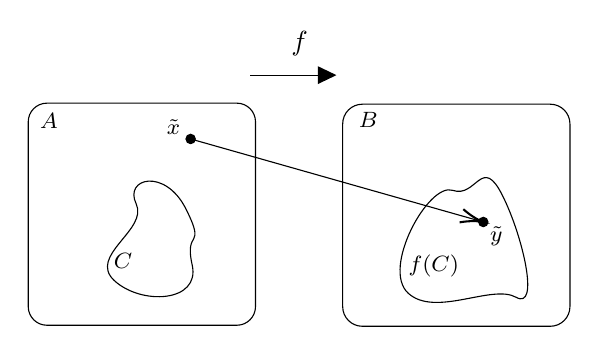
\begin{tikzpicture}[x=0.75pt,y=0.75pt,yscale=-1,xscale=1]
		%uncomment if require: \path (0,300); %set diagram left start at 0, and has height of 300
		
		%Rounded Rect [id:dp0586838643025005] 
		\draw   (50,73) .. controls (50,68.03) and (54.03,64) .. (59,64) -- (150.5,64) .. controls (155.47,64) and (159.5,68.03) .. (159.5,73) -- (159.5,162) .. controls (159.5,166.97) and (155.47,171) .. (150.5,171) -- (59,171) .. controls (54.03,171) and (50,166.97) .. (50,162) -- cycle ;
		%Rounded Rect [id:dp40936794872995397] 
		\draw   (201.5,74) .. controls (201.5,68.75) and (205.75,64.5) .. (211,64.5) -- (301.5,64.5) .. controls (306.75,64.5) and (311,68.75) .. (311,74) -- (311,162) .. controls (311,167.25) and (306.75,171.5) .. (301.5,171.5) -- (211,171.5) .. controls (205.75,171.5) and (201.5,167.25) .. (201.5,162) -- cycle ;
		%Shape: Polygon Curved [id:ds8529440642936859] 
		\draw   (102,112.5) .. controls (96,100) and (116,95) .. (126,115) .. controls (136,135) and (125,124) .. (129,142) .. controls (133,160) and (104.5,161.5) .. (91.5,149.5) .. controls (78.5,137.5) and (108,125) .. (102,112.5) -- cycle ;
		%Shape: Polygon Curved [id:ds16879268501997946] 
		\draw   (254.5,106) .. controls (266,110) and (268.5,88.5) .. (278.5,108.5) .. controls (288.5,128.5) and (296.5,164) .. (285,157.5) .. controls (273.5,151) and (246,167.5) .. (233,155.5) .. controls (220,143.5) and (243,102) .. (254.5,106) -- cycle ;
		%Shape: Circle [id:dp10126802720694927] 
		\draw  [color={rgb, 255:red, 0; green, 0; blue, 0 }  ,draw opacity=1 ][fill={rgb, 255:red, 0; green, 0; blue, 0 }  ,fill opacity=1 ] (126,81.25) .. controls (126,80.01) and (127.01,79) .. (128.25,79) .. controls (129.49,79) and (130.5,80.01) .. (130.5,81.25) .. controls (130.5,82.49) and (129.49,83.5) .. (128.25,83.5) .. controls (127.01,83.5) and (126,82.49) .. (126,81.25) -- cycle ;
		%Shape: Circle [id:dp5328965179835532] 
		\draw  [color={rgb, 255:red, 0; green, 0; blue, 0 }  ,draw opacity=1 ][fill={rgb, 255:red, 0; green, 0; blue, 0 }  ,fill opacity=1 ] (267,121.25) .. controls (267,120.01) and (268.01,119) .. (269.25,119) .. controls (270.49,119) and (271.5,120.01) .. (271.5,121.25) .. controls (271.5,122.49) and (270.49,123.5) .. (269.25,123.5) .. controls (268.01,123.5) and (267,122.49) .. (267,121.25) -- cycle ;
		%Straight Lines [id:da5038858731694382] 
		\draw    (157,50.5) -- (195.5,50.5) ;
		\draw [shift={(198.5,50.5)}, rotate = 180] [fill={rgb, 255:red, 0; green, 0; blue, 0 }  ][line width=0.08]  [draw opacity=0] (8.93,-4.29) -- (0,0) -- (8.93,4.29) -- cycle    ;
		%Straight Lines [id:da30392969256002633] 
		\draw    (128.25,81.25) -- (267.33,120.7) ;
		\draw [shift={(269.25,121.25)}, rotate = 195.84] [color={rgb, 255:red, 0; green, 0; blue, 0 }  ][line width=0.75]    (10.93,-3.29) .. controls (6.95,-1.4) and (3.31,-0.3) .. (0,0) .. controls (3.31,0.3) and (6.95,1.4) .. (10.93,3.29)   ;
		
		% Text Node
		\draw (90,135) node [anchor=north west][inner sep=0.75pt]  [font=\footnotesize] [align=left] {$\displaystyle C$};
		% Text Node
		\draw (54.5,67.5) node [anchor=north west][inner sep=0.75pt]  [font=\footnotesize] [align=left] {$\displaystyle A$};
		% Text Node
		\draw (208,67) node [anchor=north west][inner sep=0.75pt]  [font=\footnotesize] [align=left] {$\displaystyle B$};
		% Text Node
		\draw (232,136) node [anchor=north west][inner sep=0.75pt]  [font=\footnotesize] [align=left] {$\displaystyle f( C)$};
		% Text Node
		\draw (115.5,70.5) node [anchor=north west][inner sep=0.75pt]  [font=\footnotesize] [align=left] {$\displaystyle \tilde{x}$};
		% Text Node
		\draw (271.25,122) node [anchor=north west][inner sep=0.75pt]  [font=\footnotesize] [align=left] {$\displaystyle \tilde{y}$};
		% Text Node
		\draw (175.5,27.9) node [anchor=north west][inner sep=0.75pt]    {$f$};
		
		
	\end{tikzpicture}
	
	
	
\end{figure}
	